\chapter{先行研究}
\label{chap:previous}
\fancyhf{}
\rhead{\thepage}
\lhead{第\ref{chap:previous}章 先行研究}
\cfoot{\thepage}

本章では,先行研究について述べる.





\section{Massive Open Online Courses}
% - MOOCsについて,5W1Hを明らかにする
MOOCsはMassive Open Online Courses\cite{mcauley2010mooc, pappano2012year,siemens2013massive}の略称で,特に日本語で表記する場合は大規模公開オンライン講座と記述することがある.
MOOCsはオンライン上で誰もが受講できる大規模な講座群のことである.
講座を運営するプラットフォームサービスを指してMOOCsと呼ぶこともある.
MOOCsという概念の登場は2008年に主に履修登録をした学生向けに講座をオンラインで開催したら,学生だけでなく2000人以上の人がその講座に参加したことがきっかけだと言われている\cite{yuan2013moocs}.
以前から大学は
オープンコースウェア\cite{abelson2008creation}という形で講義の動画や資料を公開していたが,
MOOCsは,参加人数が非常に大規模であるという点や,高等教育水準の内容の講座だけでなく初等中等教育水準の内容の講座も含まれるという点でオープンコースウェアとは異なる.
また,これまでもオンライン講座というものは存在していたが,
MOOCsは,
参加人数が非常に大規模であるという点や
公開している講座の数が大規模である点,
また,その内容が多様であるという点,
利用が無料,あるいは無料に近いという点で,
これまでのオンライン講座とは異なる.

MOOCsではオンライン上でさまざまな講座を提供され,また各講座ごとに講義動画や演習システム,掲示板等が提供されている.
従来の教室で時間割通りに一斉授業形式で提供される学習機会とは異なり,
数多くの多様な講座のオンライン上での提供を通じて,
いつでもどこでも自分のペースでさまざまな講座から自分の学習したいものを選択し学習できるというこれまでにない学習機会を提供しており,
多くの学習者が利用している.

% - 産業や社会へのインパクト
MOOCsは場所や時間に学習ペース,内容に縛られないこれまでにない学習機会を提供しているという点で,
社会や産業への影響が期待されている.
例えば,大学生だけでなく社会人も自分の専門領域に関する講座を受講することで理解を深めたり,
あるいは,専門領域とは大きく関わりのない幅広い講座を受講することで教養を高めたりすることができる.
また,
特に,公教育の整備がまだ追いついていない発展途上国においてはMOOCsの影響は大きく,その影響や位置付け,可能性を分析する報告は多い\cite{trucano2013more,liyanagunawardena2013impact}.

% - 2,3つの事例を具体的に紹介
\begin{figure}[htb]
\begin{center}
\hspace*{-40pt}\makebox[1.2\textwidth][c]{
	\minipage{0.53\textwidth}
		
\includegraphics[width=240pt, height=180pt]{./img/cousera.png}
		\caption{Courseraのイメージ}
		\label{fig:cousera}
	\endminipage\hfill
	\minipage{0.53\textwidth}
		
\includegraphics[width=240pt, height=180pt]{./img/khanacademy.png}
		\caption{KhanAcademyのイメージ}
		\label{fig:khanacademy}
	\endminipage\hfill
}
\end{center}
\end{figure}
MOOCsの有名な事例としては,Coursera\footnote{\url{https://www.coursera.org/}}やKhan Academy\footnote{\url{https://www.khanacademy.org/}}が挙げられる.
MOOCsとKhan Academyのイメージを図\ref{fig:cousera},\ref{fig:khanacademy}に示す.
Courseraは主に大学の講座を提供するMOOCsで2016年1月の時点で,
コンピュータサイエンス,数学や論理,社会科学などに関する1500以上の講座を提供し,世界中から1700万人以上が利用している\footnote{講座数と利用者数はトップページの記載より引用.}.
図\ref{fig:cousera}では,データサイエンス,ビッグデータ,機械学習,ビジネスアナリティクス等の講座が人気講座として表示されているが,このように提供されている講座は専門性が高いものも多い.
Khan Academyは2008年にサービスを開始し,主に初等中等教育水準の講座を提供するMOOCsで2016年1月の時点で,
数学,生物,芸術史,地理などに関する多くの講座を提供し,また,演習問題については10万以上が提供されており\footnote{トップページの記載より引用.},世界中の学習者が利用している.
初等中等教育水準の講座への提供ということもあり,図\ref{fig:khanacademy}にあるように保護者や先生と連携する仕組みもある.




% - マトリックスでMOOCsの分類を提示
MOOCsはそのプラットフォームや運営者に応じて内容や性質が異なり,それらを体系化する研究も多い.
\cite{yuan2013moocs}では,MOOCsを4つの項目
1) サービスが営利目的か否か,
2) アクセスが有料か否か,
3) 修了証が有料か否か,
4) 単位取得できるか否か,
で整理した.
この整理では,
例えば,Courseraは営利目的のサービスであり,アクセスは無料で,修了証の発行は有料で,単位取得は一部可能というように整理される.
また,MOOCsの設計の背後にある教育学的立場の違いからしばしばxMOOCsとcMOOCsに分けて議論される\cite{daniel2012making}.
cMOOCsはconnectivist MOOCsの略称で学習者間のやり取りを通した学習を重視したMOOCsであり,
xMOOCsはコンテンツベースの学習を重視したMOOCsである.



% - 当初の期待よりは影響がなかった.
このように,MOOCsは,その登場より多くの学習者が利用しており期待も高かったが,
MOOCsはその登場当初に期待されていたほど,教育や学習に効果があったというわけではない.
特に,MOOCsにおける大きな課題の1つとして学習の継続性が非常に低いということが挙げられる.
さまざまなMOOCsで提供されている講座の受講完了率を集計した報告
\cite{jordan2013mooc}によると,
MOOCsの講座完了率は15\%程度であるという.
また,\cite{rivard2013measuring}によると,
Courseraで提供されたデューク大学の生体電気に関する講座の履修状況は
当該講座に履修登録した12,700人の受講者の中で,最終テストを受けた受講者は350人と全体の3\%程度だったという.
これまでにない学習の機会を提供しているという点で非常に期待されていたが,
継続的に勉強しなければ継続的な学習効果は期待できず,
したがって,学習の継続性が低いということはMOOCsにおける大きな課題であるといえる.

また,初等中等教育への影響に懐疑的な意見もある.
学習者のやる気や多様性の観点から考察して報告した研究\cite{bock2013virtual}では,
オンライン学習はやる気の強い学習者にとってはよく機能するがそうでない学習者は辞めてしまうことや,
異なる教育背景を持つ多様な学習者に対応できるだけの柔軟性がまだMOOCsにないが,特に初等中等教育水準の学習ではそれが重要であることが
が指摘された.


% - 学習行動データの分析可能性の拡大
MOOCsはこうした学習者に学習の機会を提供するという側面だけでなく,
これまで難しかった大規模な学習効果分析の可能性を高めるという側面もある.
学習者はオンライン上で提供された講義動画や演習問題を通して学習するが,
オンライン上で実施されているため学習行動ログをデータとして蓄積することができ,さらに,そのデータを分析に活用することができる.
また,多くの多様な学習者が利用するため,多様な学習者の大規模な学習行動ログから多様な講座の学習効果の分析が可能となりつつある.
特に,演習問題の回答ログはその演習問題により評価される知識を学習者が獲得しているか否かを表現しているため,知識獲得の分析に利用できる.
例えば,MOOCsの演習問題の回答ログを利用して知識獲得の予測を行う研究\cite{machardy2015toward}では,
Khan Academyから収集したデータを利用していたが,
その問題回答ログ数は100万件以上であり,
これまでにないほど大規模なデータを対象に分析が実施されたといえる.

% - 学習効率の向上のための知識獲得の予測と,それに基づいた教材推薦システムの開発は効果が大きい.
また,MOOCsは多くの学習者が利用しており,こうした分析に基づいた学習の効率化や学習の継続を促進する教材推薦システムの開発は効果大きいと考えられる.
従来,eラーニングによる学習支援システムは,
例えば大学であれば大学に所属する学生が利用者の中心で大学に所属していない人の利用が難しかったように,
学習支援システムの利用者が限定されており,したがって,教材推薦による学習の効率化の活用可能性も限定的であったと考えられる.
しかし,MOOCsにおける学習効果の改善は,単に一部の限られた学習者がその恩恵を享受できるということに留まらず,
世界中の幅広い利用者がその恩恵を享受できるため,その社会的な影響は小さくないと考えられる.


\vvspace
以上,MOOCsについて述べた.
次に,深層学習について述べる.


\section{深層学習}
% - 深層学習の5W1Hについて説明
深層学習は多層のニューラルネットワークによる機械学習のことで,
従来の機械学習では難しかった対象データの抽象的表現の抽出を最適化の過程で行うことができる.
深層学習の活用により画像認識\cite{schroff2015facenet,szegedy2014going},音声認識\cite{hinton2012deep, bahdanau2015end},会話認識\cite{sak2015fast},機械翻訳\cite{sutskever2014sequence, dong2015multi},質問応答文生成\cite{yin2015neural},画像説明文生成\cite{xu2015show,vinyals2014show}等さまざまな研究領域で飛躍的な進展が報告がされている.

% - 深層学習の驚異的事例について2, 3説明
画像認識では深層学習により例えば犬の表現として目や鼻,口の表現が抽出できると報告する研究\cite{zeiler2014visualizing}や,
人間より高い精度で人の顔を見分けられたと報告する研究\cite{schroff2015facenet}もある.
また,機械翻訳の領域では,翻訳前の文章の長さと翻訳後の文章の長さが可変の場合でも利用でき,文章の長さに依らない特徴を抽出する機械翻訳モデルを開発し,英語からフランス語への翻訳を試みる研究\cite{sutskever2014sequence}や
フランス語とオランダ語,スペイン語の共通表現を抽出し英語からただ1つのモデルで3言語に翻訳する研究もある\cite{dong2015multi}.
また,これらを掛け合わせた画像説明文生成の領域では,説明文の単語1つずつを生成する際に画像のどの部分に着目すべきかという表現を抽出し,説明文を生成する研究\cite{xu2015show}もある.
このように,深層学習は多くの研究領域で大きな進展をもたらしている.

%大規模データが必要であることに言及
深層学習モデルを学習させるときには,大規模な訓練データが必要となる.
深層学習モデルの内部変数は非常に膨大で数十万や数百万以上となることも多く,
膨大な変数を学習させるためには,通常,大規模な訓練データが必要である.
例えば,
人間より高い精度で人の顔を見分けらると報告する顔認識の研究\cite{schroff2015facenet}では,
数百万人の2億枚以上の顔画像を訓練データに利用している.
英語からフランス語に翻訳する機械翻訳の研究\cite{xu2015show}では,
1200万もの文章を訓練データとして利用している.



% - 特に,知識獲得の予測で用いられるRNNについて5W1H
深層学習のネットワークには,いくつかの種類があるが,特に,画像処理に利用されるConvolutional Neural Networks\cite{lecun1998gradient}というネットワークと系列データの処理に利用されるRecurreut Neural Networks\cite{williams1989learning}(以下,RNN)というネットワークがよく利用される.
ここでは,知識獲得の予測に深層学習を用いた手法\cite{piech2015deep}に用いられていたニューラルネットワークであるRNNについて説明する.
%RNNは深層ニューラルネットワークの一種で主に系列データの解析に利用される.


% - RNNがよく使われる事例について紹介
近年,RNNはデータの大規模化や計算機性能の向上などにより幅広い領域の系列データに対して適用されるようになった.
具体的には,
機械翻訳\cite{sutskever2014sequence, dong2015multi},手書き文字認識\cite{graves2009offline,louradour2014curriculum},音声認識\cite{hinton2012deep,bahdanau2015end},ユーザログ解析\cite{hidasi2015session},画像説明文生成\cite{xu2015show,vinyals2014show},医療診断\cite{choi2015doctor,lipton2015learning}等の領域で高い性能を発揮することが報告されている.

% - RNNの構造の概略
\begin{figure}[htb]
\begin{center}
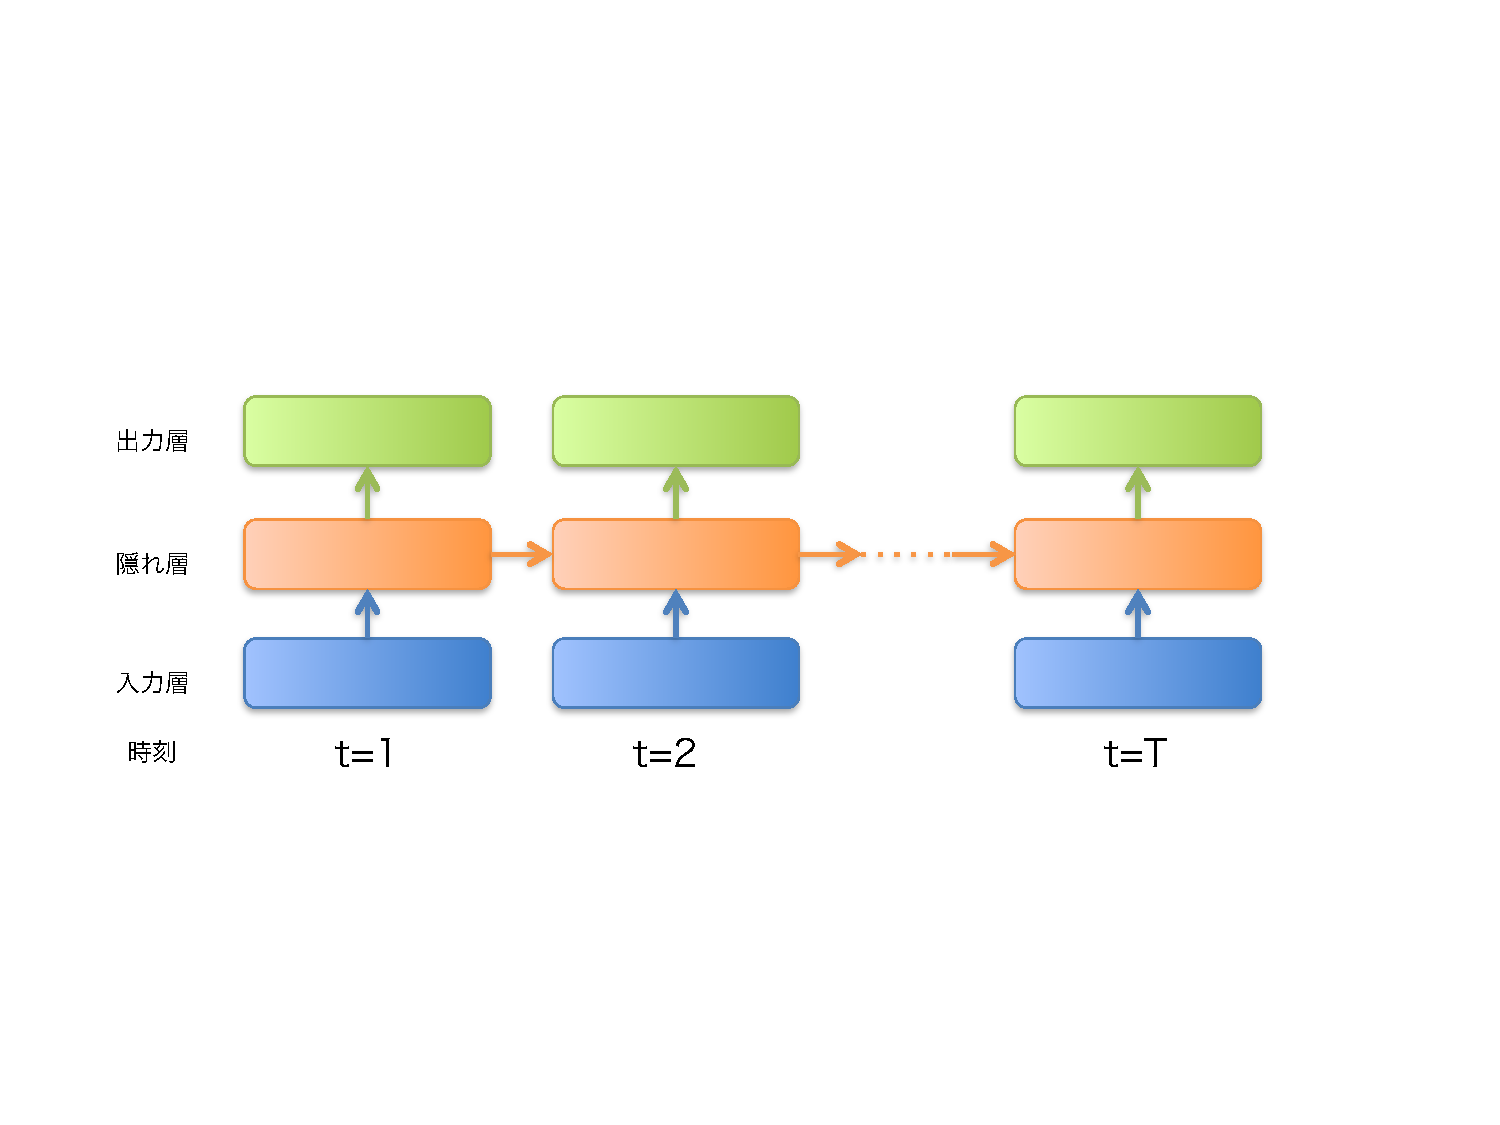
\includegraphics[width=350pt]{./img/RNN4.pdf}
\end{center}
\caption{RNNの構造のイメージ}
\label{fig:RNN}
\end{figure}
伝統的なRNNの構造は図\ref{fig:RNN}のように,
入力層,隠れ層,出力層の3層から構成されている.
系列方向を時刻とすれば,
時刻$t$の隠れ層${\bf h}_t$の計算に時刻$t-1$の隠れ層の情報を入力する${\bf h}_t = f({\bf x}_t, {\bf h}_{t-1})$の式ように,一つ前の情報を繰り返し(recurrent)入力するという構造である.
関数$f$は,入力である${\bf x}_t$や${\bf h}_{t-1}$をアフィン変換して足しあわせた後,活性化関数にかけるというものがよく利用される.
活性化関数はシグモイド関数やtanh(Hyperbolic Tangent関数),Relu\cite{nair2010rectified},ELUs\cite{clevert2015fast}など多く提案されており,通常,非線形関数である.



% - RNNの課題について説明
RNNの1つの特徴として,効果的に長期的な表現を学習させることが難しいということが挙げられる\cite{bengio1994learning}.
RNNの学習には勾配法に基づいた確率的勾配降下法\cite{robbins1951stochastic,kushner2003stochastic}やAdam\cite{kingma2014adam},AdaDelta\cite{zeiler2012adadelta}など,さまざまな手法が利用可能である.
しかし,いずれの勾配法を用いるにせよ,
勾配が爆発して学習モデルが壊れてしまうという勾配爆発\cite{bengio1994learning,pascanu2013difficulty}という問題や,
勾配が消滅して対象データの長期的な特徴量を捉えることができないという勾配消滅\cite{pascanu2013difficulty, hochreiter1998vanishing}という問題がしばしば発生する.
これは,
${\bf h}_t = f({\bf x}_t, {\bf h}_{t-1})$の式に表れるように同じ変換を繰り返し行うためであり,
このため,特に,長い系列データをRNNで学習する場合,効果的に長期的な表現を学習させることが難しい


% - 課題解決の手法について説明
こうした問題を解決もしくは緩和するため,ゲート付き活性化関数の利用や学習時の勾配に制約を加える方法が提案されている.
勾配消滅の緩和に対しては,ゲート付き活性化関数の利用が有効であるが,詳細は後述する.
勾配爆発の緩和に対しては,学習時の勾配に制約を加える方法が有効である.
具体的には,
\cite{mikolov2012statistical}では
学習させるパラメタの勾配の絶対値の最大値を予め決めておき,
最大値以上の場合には,勾配の最大値になるように勾配の値を置き換えることで勾配爆発の影響を緩和する方法が報告された.
また,
\cite{pascanu2013difficulty}では
学習させるパラメタの勾配のノルムの最大値を予め決めておき,
最大値以上の場合には, ノルムが最大値以下になるように疑似コード\ref{normregular}に従いノルムを抑制することで勾配爆発の影響を緩和する方法が報告された.
\begin{algorithm}                      
\caption{勾配爆発を防ぐための勾配ノルム抑制の疑似コード}
\label{normregular}                          
\begin{algorithmic}                  
	\STATE $\hat{{\bf g}} \leftarrow \frac{\delta \varepsilon}{\delta {\bf \theta}}$
	\IF{$\Vert \hat{{\bf g}} \Vert \geq threshold $}
	\STATE $\hat{{\bf g}} \leftarrow \frac{threshold}{\Vert \hat{{\bf g}} \Vert} \hat{{\bf g}}$
	\ENDIF
\end{algorithmic}
\end{algorithm}


先に,言及したが,RNNには異なる活性化関数を利用するという形でいくつかの種類がある.うまく設計された活性化関数を利用することで,データの長期的な特徴をよく捉えられたり,計算コストを削減することができたりする.以降では,よく研究報告で取り上げられるSimple RNN(以下,SRNN)\cite{williams1989learning},Long Short  Term Momory RNN(以下,LSTM-RNN)\cite{hochreiter1997long},Gated Recurrent Neural Networks(以下,GRNN)\cite{cho2014learning}の3つについて詳細に説明する.

% - SRNN

% - LSTM-RNN

% - GRNN





\subsubsection{SRNN}
SRNNはゲート付き活性化関数を用いない簡単な構造のRNNである.
\cite{le2015simple, krueger2015regularizing}で報告される工夫を取り入れることで,データの長期的な特徴を効果的に捉えることができるようになるが,
多くの場合で,LSTM-RNNやGRNNのようにゲート付き活性化関数を用いるRNNの方がモデルの性能という点で優れている.

SRNNによるモデルの定式はいくつか種類が存在するが,シンプルなものは例えば下記の式で定義される.
\begin{eqnarray}
\label{eq:srnn1}
{\bf h}_t &=& \tanh({\bf W}_{xh} {\bf x}_t + {\bf W}_{hh}  {\bf h}_{t-1} + {\bf b}_h)\\
\label{eq:srnn2}
{\bf y}_t &=& \sigma( {\bf W}_{hy} {\bf h}_t + {\bf b}_y)
\end{eqnarray}
ここでは,
$t$は時刻を指し,
${\bf x}_t$は時刻$t$の入力ベクトルを指し,
${\bf h}_t$は時刻$t$の隠れ層を指し,
${\bf y}_t$は時刻$t+1$の各問題の正誤確率の予測値を指し,
${\bf W}_{xh}$,${\bf W}_{hh}$はそれぞれ重み行列を指し,
${\bf b}_h$,${\bf b}_y$はそれぞれバイアス項を指し,
$\tanh$は$( e^x - e^{-x} )/( e^x + e^{-x} )$で定義されるHyperbolic Tangent関数を指し,
$\sigma$は$1 / (1 + e^{-x})$で定義されるシグモイド関数を指す.
訓練時には,重み行列${\bf W}_{xh}$,${\bf W}_{hh}$とバイアス項${\bf b}_h$,${\bf b}_y$を学習する.



\vvspace
以上,深層学習について述べた.
次に,知識獲得の予測について述べる.





\section{知識獲得の予測}
% - 知識獲得の予測について5W1H(what, when, who, why, where, how)
知識獲得の予測は,学習者が対象の知識を獲得しているか否かを予測する問題である.
通常,知識を獲得しているか否かは問題回答の正誤を基に評価されるため,
知識獲得の予測のタスクは過去の学習者の問題回答履歴から次に解く問題の正誤を予測するというものである.
最初の定式化の事例は,1994年にCorbettらによって報告されたKnowledge Tracing\cite{corbett1994knowledge}である.
スキルの習熟学習において,
領域知識をよく分析し階層的に知識間関係を構築し,
階層構造においてより水準の高い知識に着手する前に予め獲得するべき知識が確実に獲得されるように学習体験を設計することで,
ほとんどの学習者がスキルを十分に習熟できるとする仮説\cite{keller1968good, bloom1968learning}や,
コンピュータサイエンスの発展を受けて,
予め獲得すべき知識が確実に獲得されるように学習者の知識の獲得有無を予測するというのが主な目的であった.
Knowledge Tracingにおける学習者とモデルは,学習者が勉強し知識を獲得したら,モデルが学習者が獲得した知識を予測することで学習者の獲得している知識の変化を追跡する({\it Knowledge Tracing}),という関係になっている.


% - 伝統的には2つのアプローチがあることを説明
伝統的に,知識獲得の予測には知識獲得の時系列性を重視するものと,知識間の関係性を重視するものがある.
\cite{corbett1994knowledge}で報告されたBayesian Knowledge Tracingという手法は知識獲得の時系列性を重視するもので,
問題に予めスキルを割り当て個々のスキルに習熟過程に関する4つの確率変数を定義しモデル化するというもので,
スキル間の関係性は考慮しないが,個々のスキルの習熟,つまり時系列性を考慮する手法である.
\cite{pavlik2009performance}で報告されたPerformance Factor Analysisという手法は知識間の関係性を重視するもので,
個々の知識(あるいは,スキル)に関する過去の回答の正誤を重み付けして,次の問題の正誤を予測しようというもので,
Performance Factor Analysisは知識獲得の時系列性より知識間の関係性を重視する手法である.
いずれの手法も本論文と関連が深い.


以降では,まず,Knowledge Tracingの定式化について述べ,
Bayesian Knowledge TracingとPerformance Factor Analysisの2つの手法を説明し,
最後に,深層学習を活用したDeep Knowledge Tracingについて説明する.



% - Knowledge Tracing

% - Bayesian Knowledge Tracing

% - Performance Factor Analaysis

% - Deep Knowledge Tracing





\subsection{Knowledge Tracingの定式化}
Knowledge Tracingは過去の学習者の問題回答履歴から学習者が次に解く問題の正誤を予測するというものである.
学習者の時刻$t$において観測された問題回答結果を$q_{t}$とすれば,
$q_1, q_2, \dots, q_t$から時刻$t+1$において観測される問題回答結果$q_{t+1}$を予測するタスクと表現できる.
特に,過去の観測された問題の正誤から将来の正誤確率を算出する場合は,
$q_1, q_2, \dots, q_t$が観測された場合の時刻$t+1$に着手する問題において当該学習者の回答正解となる事後確率
$p(q_{t+1} = correct|q_1, q_2, \dots, q_t)$を求めるタスクであるといえる.
予測性能の評価は\cite{yudelson2013individualized, falakmasir2015spectral}ではAccuracyで,\cite{piech2015deep}ではAUCで行っており,
目的に応じてさまざまである.

なお,モデルの入力次元である{\bf 問題}の粒度はさまざまである.
問題はその問題を回答するのに必要な知識を学習者が獲得しているか否かを評価するという点で,
問題は知識集合を表現していて,また,その粒度もさまざまである.
個々の問題をそのままモデルの入力次元とするものや,問題に予めタグを割り当て問題により評価される知識の粒度をある程度整え,そのタグをモデルの入力次元とすることもある.
例えば,
\cite{piech2015deep}ではモデルの入力次元は演習タグもしくはスキルタグと呼ばれるものであり,
演習問題に割り当てられ,それぞれの演習問題で扱われる学習要素を説明するものである.
通常,こうしたタグは専門家によって設計され,利用される.
本論文では個々の問題をそのままモデルの入力次元として用いる.


\subsection{Bayesian Knowledge Tracing}
Bayesian Knowledge Tracing\cite{corbett1994knowledge}(以下,BKT)はベイズの定理の事前確率と事後確率の関係に基づいて正解確率$p(q_{t+1} = correct|q_1, q_2, \dots, q_t)$をモデリングする手法である.
BKTには下記の4つの確率変数がある.
\begin{itemize}
\item 初めから当該スキル理解している確率$p(L_0)$(もしくは $p\mhyphen init$)
\item 学習者が当該スキルを理解していない状態から理解している状態へ遷移する確率$p(T)$(もしくは $p\mhyphen transit$)
\item 学習者が当該スキルを理解しているが誤答する確率$p(S)$(もしくは $p\mhyphen slip$)
\item 学習者が当該スキルを理解していないが推測で正解する確率$p(G)$(もしくは $p\mhyphen guess$)
\end{itemize}
これらの4つの確率変数がすべてのスキルに定義されている.つまり,スキル数を$N$とすれば,確率変数の合計数は$4N$である.
学習者$u$がスキル$k$の問題を時刻$t$に解いた場合に正解する確率は下記の式に基づいて更新される.

\hspace*{-55pt}\minipage{1.1\textwidth}
\begin{eqnarray}
\label{eq:bkt_update1}
p(L_1)^{k}_{u} &=& p(L_0)^k \\[\eqnsp]
\label{eq:bkt_update2}
p(L_{t}|obs=correct)^{k}_{u} &=& \frac{ p(L_{t-1})^{k}_{u} \cdot (1 - p(S)^k) }{ p(L_{t-1})^{k}_{u} \cdot (1 - p(S)^k) + (1 - p(L_{t-1})^{k}_{u}) \cdot p(G)^k } \\[\eqnsp]
\label{eq:bkt_update3}
p(L_{t}|obs=wrong)^{k}_{u} &=& \frac{ p(L_{t-1})^{k}_{u} \cdot p(S)^k }{ p(L_{t-1})^{k}_{u} \cdot p(S)^k + (1 - p(L_{t-1})^{k}_{u}) \cdot (1 - p(G)^k) } \\[\eqnsp]
\label{eq:bkt_update4}
p(L_{t})^{k}_{u} &=& p(L_{t}|obs)^{k}_{u} + (1 - p(L_{t}|obs)^{k}_{u}) \cdot p(T)^k  \\[\eqnsp]
\label{eq:bkt_update5}
p(C_{t})^{k}_{u} &=& p(L_{t-1})^{k}_{u} \cdot (1 - p(S)^k) + (1 - p(L_{t-1})^k_{u}) \cdot p(G)^k
\end{eqnarray}
\endminipage\hfill
%}
\vvspace
\vvspace


右上の$k$はスキル番号を示し,右下の$u$はユーザ番号を示すことに注意されたい.
まず,学習者$u$が初めから当該スキル$k$を身につけている確率は式\ref{eq:bkt_update1}の通り定義する.
正解が観測され,正しく当該スキルを身につけている確率は,式\ref{eq:bkt_update2}で与えられ,
不正解が観測されたが,正しく当該スキルを身につけている確率は,式\ref{eq:bkt_update3}で与えられ,
それらを合わせて,次の時刻に当該スキルを身につけている確率は,式\ref{eq:bkt_update4}で与えられる.
このように定めることで,理解しているがうっかり間違ってしまう場合や, 理解していないがあてずっぽうで正解してしまう場合を考慮できる.
なお当該モデルでは,身につけたスキルの忘却は無視している.
最後に,学習者$u$がスキル$k$の問題を時刻$t$に解いた場合に正解する確率$p(C_{t})^{k}_{u}$は式\ref{eq:bkt_update5}のように算出され,
この値を次の問題の正誤予測に利用する.
 
上記に説明したモデルの学習にはいくつかの方法が適用され報告されている.
1つは\cite{corbett1994knowledge}にあるようにHMMを用いて生成モデルとして学習させる方法であり,
1つは\cite{yudelson2013individualized}にあるように勾配法を用いて識別モデルとして学習させる方法である.
それぞれ長所と短所があるが,
特に,大規模データへの適用という観点ではHMMに基づいた生成モデルの手法では計算量が大きく学習に非常に多くの時間がかかってしまうということもあり,
\cite{yudelson2013individualized}では勾配法に基づいた識別モデルとして学習させている.
具体的には,\cite{yudelson2013individualized}では,目的関数に負の対数尤度(Negative Log Likelihood)を利用し,勾配降下法(Gradient Descent)で学習させている.
%本論文で扱うデータは大規模であるため,学習方法は識別モデルとして扱う場合について説明した.
%生成モデルとして扱う場合の学習方法については\cite{corbett1994knowledge}を参照されたい.



\subsection{Performance Factor Analysis}
Performance Factor Analysis\cite{pavlik2009performance}(以下,PFA)も
過去の学習者の問題回答履歴から学習者が次に解く問題の正誤を予測するための手法である.
しかし,
知識獲得の時系列性を考慮するBKTと異なり,
知識獲得の順番を考慮せず知識間の関係性を考慮して予測する手法である.
PFAは下記のように定義される.
\begin{eqnarray}
	p(i, j \in KCs, s, f) & = & \sigma( \beta _j + \sum_{k \in KCs}(\gamma_k s_{i, k} + \rho _k f_{i, k}) )
\end{eqnarray}
ここでは,
$s$は事前に正答した問題回答,
$f$は事前に誤答した問題回答,
$p$はユーザ$i$が知識$j$に正答する確率,
$\beta_j$は知識$j$の簡単さ,
$\gamma_k$と$\rho_k$はそれぞれ知識$k$の正答と誤答の重み,
$s_{i, k}$と$f_{i, k}$はそれぞれユーザ$i$が知識$k$に事前に正答した問題回答,事前に誤答した問題回答
である.
$\sigma$はシグモイド関数,
過去の各知識の正誤を重み付けしシグモイド関数にかけ,別の問題の正誤を予測するというものである.

%特に,深層学習を用いる前のKnowledge Tracingでは
%問題回答の順番を考慮していたが知識間の関係性は考慮する研究は著者の知る限り\cite{kaser2014beyond}の以外ない.
PFAは
知識間の関係性を考慮できない場合に複数の知識がないと獲得できない知識のモデルが難しいという
Bayesian Knowledge Tracingやその拡張手法の問題を解決するために
提案された.
PFAは知識間の関係性を重み付けして考慮しているが,
問題回答の順番は考慮しない.


\subsection{Deep Knowledge Tracing}
Deep Knowledge Tracing\cite{piech2015deep}(以下,DKT)はRNNを利用しKnowledge Tracingを行う手法である.
2015年6月に発表された.
数学の問題回答ログのデータセットで実験され,
高い性能で将来の知識獲得を予測できること,
予測モデルを分析することで知識間関係をネットワークとして抽出できることが報告された.
学習者が獲得している知識から,ある知識の獲得されやすさをそのまま予測しており,
得られた知識間関係から抽出されたネットワークは知識獲得における知識構造を表現しているといえる.
DKTの構造と最適化,および知識間関係の抽出手法について順に説明していく.



\subsubsection{構造}
まず,DKTの構造について述べる.
DKTの構造は伝統的なRNNの構造に基づいている.
伝統的なRNNは入力のベクトル系列${\bf x}_1, \dots, {\bf x}_T$を出力のベクトル系列${\bf y}_1, \dots, {\bf y}_T$に写像する.
この写像は,隠れ状態${\bf h}_1, \dots, {\bf h}_T$を計算することで達成されるが,一連の写像の過程で過去観測から得られる関連情報を将来予測のために連続的に符号化している,とみなせる.確率変数は下記の式で定義されるネットワークにより関連付けられる.
\begin{eqnarray}
\label{eq:rnn1}
{\bf h}_t &=& f({\bf x}_t, {\bf h}_{t-1})\\
\label{eq:rnn2}
{\bf y}_t &=& g({\bf h}_t)
\end{eqnarray}
モデルは関数$f$と$g$によって定義されており,
これらの関数$f, g$にはSRNNの式\ref{eq:srnn1},\ref{eq:srnn2}やLSTM-RNNの式\ref{eq:lstmrnn1}--\ref{eq:lstmrnn7},GRNNの式\ref{eq:grurnn1}--\ref{eq:grurnn5}を利用できる. 


RNNで学習者の学習行動の観測結果をモデリングするため観測結果を固定長の入力ベクトル${\bf x}_t$の系列に変換する必要があるが,DKTではシンプルな変換を行っている.具体的には,学習者の学習行動の観測結果をone-hotベクトルに符号化し${\bf x}_t$とする,というものである.
観測結果は演習問題と正誤の組み合わせで表現できるため,演習問題の数を$M$とすれば,${\bf x}_t$の長さは$2M$となる.


\begin{table}[ht]
\caption{Deep Knowledge Tracingにおける回答ログデータと対応する入力ベクトルの例}
\label{tab:samplelog}
\begin{center}
\centerline{
{
\begin{tabular}{crrr|cc}\hline\hline
	\multicolumn{4}{c|}{回答ログ}	&	\multicolumn{2}{c}{入力ベクトル}	\\
	ユーザID	&	ログの順番	&	問題番号	&	正誤	&	変数名			&	値											\\\hline
	A			&	1			&	1			&	0		&	${\bf x}_1$ 			& $[0 0 0 0 \vdots 1 0 0 0 ]$	\\
	A			&	2			&	1			&	1		&	${\bf x}_2$ 			& $[1 0 0 0 \vdots 0 0 0 0 ]$	\\
	A			&	3			&	2			&	1		&	${\bf x}_3$ 			& $[0 1 0 0 \vdots 0 0 0 0 ]$	\\
	A			&	4			&	3			&	0		&	${\bf x}_4$ 			& $[0 0 0 0 \vdots 0 0 1 0 ]$	\\
	A			&	5			&	3			&	1		&	${\bf x}_5$ 			& $[0 0 1 0 \vdots 0 0 0 0 ]$	\\
	A			&	6			&	4			&	1		&	${\bf x}_6$ 			& $[0 0 0 1 \vdots 0 0 0 0 ]$	\\
\hline\hline
\end{tabular}
}
}
\end{center}
\end{table}


具体例を交えて説明する.
例えば,演習問題の数が4つで,問題回答は1つずつしかできないと仮定する .$M=4$であり,${\bf x}_t$の長さは$8$である.
ある学習者が,表\ref{tab:samplelog}の回答ログように問題を回答し正誤が観測されたとする.
この時に,例えば,表\ref{tab:samplelog}に記載のような入力ベクトルの系列となる.
このようにして,回答行動の観測結果を符号化することで,どの演習問題をいつ正解もしくは不正解したのかをRNNに入力できる.

出力${\bf y}_t$は問題と同じ長さのベクトルで,
それぞれの要素が当該学習者がそれぞれの問題に正しく回答する確率の予測値となっている.
したがって,$t+1$の回答$q_{t+1}$の正誤予測は$t+1$に回答される問題$q_{t+1}$に対応する${\bf y}_t$の要素から読み取れる.


\subsubsection{最適化}
次に,DKTの最適化について述べる.
訓練時に用いられる目的関数は,
モデルにおいて学習者の回答行動の観測系列の負の対数有度(Negative Log Likelihood)である.
${\bf \delta}(q_{t+1})$を時刻$t+1$にどの問題が回答されたかのone-hotベクトルとし,
$a_{t+1}$を時刻$t+1$に当該問題で正答したか否か($1$か$0$)とし,
$l$をクロスエントロピーとすれば,
当該予測結果に対するロス関数は $l({\bf y}^T {\bf \delta}(q_{t+1}), a_{t+1})$であり,
学習者一人のロスは下記の式で与えられる.
\begin{eqnarray}
L &=& \sum_t l({\bf y}_t^T {\bf \delta}(q_{t+1}), a_{t+1})
\end{eqnarray}


学習時はミニバッチごとに確率的勾配降下法で目的関数を最小化する.
\cite{piech2015deep}では,モデル学習時には過学習を防ぐため${\bf y}_t$への入力としての${\bf h}_t$にはdropout\cite{srivastava2014dropout}を適用している(${\bf h}_{t+1}$の方向にはdropoutを適用しない).
また,系列方向の誤差逆伝搬\cite{werbos1990backpropagation}において勾配が爆発するのを防ぐため,閾値以上のノルムの勾配は\cite{pascanu2013difficulty}にしたがい,制約を設けている.


\subsubsection{知識間関係抽出法}
次に,DKTのモデルを利用した知識間関係(あるいは,問題間関係)抽出法について述べる.
DKTのモデルは,従来ではよく人間の専門家が行っていたデータの潜在的な構造や概念を発見するタスクに応用できる.
問題$i$と$j$のすべての有向ペアのうち下記の条件を満たすものに対して下記の影響度$J_{ij}$を割り当てる.\\
\begin{itemize}
	\item [条件]有効ペア$(i, j)$について,問題$i$が出現した後に残りの問題系列の中で問題$j$が出現する系列数が問題$i$が出現する問題系列数全体の$V\%$以上であること.
	\item[影響度]
$$J_{ij} = \frac{y(j|i)}{\sum_k y(j|k)}$$\\
\end{itemize}
ここでは,$y(j|i)$は,ある学習者が最初に問題$i$に正答した場合に,RNNによって割り当てられる次の時刻に問題$j$に正答する確率である.
\cite{piech2015deep}では,問題間影響行列からのネットワーク抽出には,
$V=1$を用いた.
また,ネットワークの可視化に際しては,影響度が$0.1$以上であればエッジを引くというようにしてネットワークを構築した.

さらに,\cite{piech2015deep}は,
得られたネットワークは,
単に学習者の問題$(i, j)$間の遷移率から構築したネットワークや
問題$i$の正解が観測された後に問題$j$の正解が観測される条件付き確率から構築したネットワークより
よく知識間関係を捉えていることを指摘している.


こうして得られた行列$J$は,
問題$i$で評価される知識が既に獲得されている場合に,
問題$j$で評価される知識の獲得されやすさを表現しており,
$J$は知識間関係行列であるといえ,
この知識間関係行列から構築したネットワークは
知識獲得における知識構造を表現していると考えられる.


\vvspace
以上,知識獲得の予測について述べた.
次に,ネットワーク分析について述べる.

\section{ネットワーク分析}




\vvspace
以上,先行研究について述べた.
次に,分析手法について述べる.




